\documentclass{report}

\usepackage[utf8]{inputenc}
\usepackage{graphicx}
\usepackage[margin=35mm]{geometry}
\usepackage[colorlinks = true,linkcolor = red, urlcolor  = blue, citecolor = blue, anchorcolor = blue]{hyperref}
\usepackage[pagestyles]{titlesec}
% Load the package with the acronym option
\usepackage[automake]{glossaries}
\usepackage[section]{placeins}
 \usepackage{lipsum}
\usepackage{wrapfig}
\usepackage{titling}
\usepackage{caption}
\usepackage{enumitem}
\usepackage{listings}
\usepackage{pythontex}
\usepackage{algorithm}
\usepackage{amsmath}
\usepackage{algpseudocode}
\usepackage{varwidth}
\usepackage{xpatch}
\usepackage{fancyhdr}
\usepackage[backend=bibtex,style=numeric,sorting=none]{biblatex}
\usepackage{hyperref}


\fancyfoot[C]{\thepage} 
\addbibresource{bibresource.bib}  

\titleformat{\chapter}[display]
    {\normalfont\huge\bfseries}{\chaptertitlename\ \thechapter}{20pt}{\Huge}
\titlespacing*{\chapter}{0pt}{-30pt}{20pt}

\titleformat{\chapter}%
  {\normalfont\bfseries\LARGE}{\thechapter.}{10pt}{}

\titleformat{\section}%
  {\normalfont\bfseries\large}{\thesection.}{10pt}{}

\titleformat{\subsection}%
  {\normalfont\bfseries\small}{\thesubsection.}{10pt}{}

\renewcommand*{\glstextformat}[1]{\textcolor{black}{#1}}
% Acronym definitions

\newacronym{DoS}{DoS}{Denial-of-Service attack}
\newacronym{DDoS}{DDoS}{Distributed Denial-of-Service attack}
\newacronym{OSI}{OSI}{Open Systems Interconnection}
\newacronym{SSL}{SSL}{Secure Sockets Layer}
\newacronym{TCP}{TCP}{Transmission Control Protocol}
\newacronym{ICMP}{ICMP}{Internet Control Message Protocol}
\newacronym{APDoS}{APDoS}{The Advanced Persistent Denial-of-Service}
\newacronym{SNMP}{SNMP}{Simple Network Management Protocol}
\newacronym{CDN}{CDN}{Content Delivery Network}
\newacronym{UDP}{UDP}{User Datagram Protocol}
\newacronym{IP}{IP}{Internet Protocol}
\newacronym{IPS}{IPS}{Intrusion Prevention System}
\newacronym{MAC}{MAC}{Media Access Control}
\newacronym{ISP}{ISP}{Internet Service Providerl}
\newacronym{SDN}{SDN}{Software-Defined Networking}
\newacronym{HTTP}{HTTP}{Hypertext Transfer Protocol}
\newacronym{NS}{NS}{Network Simulator}
\newacronym{GUI}{GUI}{Graphical User Interface}

\makeatletter
\xpatchcmd{\algorithmic}{\itemsep\z@}{\itemsep=1ex plus2pt}{}{}


\makeatother
%\pretitle {
 % \begin{center}
 % \LARGE
  %\includegraphics[width=6cm,height=2cm]{arielLogo}\\[\bigskipamount]
%}
%\posttitle{\end{center}}
% Generate the glossary
\makeglossaries

\title{Automatically defend from DoS and DDoS traffic flood attacks}
\author{Yinon Cohen and Maor Shabtay\\\\{ Advisor: Dr. Amit Dvir}\\\\{Ariel University}}
\date{September 2018}

\begin{document}
\maketitle
\tableofcontents
\addtocontents{toc}{~\hfill\textbf{Page}\par}


\newpage

\chapter {Abstract}
\hfill \break \gls{DoS} and \gls{DDoS} attacks are attempts to exhaust server side assets, and designed to prevent client-to-server communication (denial of service). These attacks aim to both public and private sectors, and occur more and more frequently. In addition, lately the massive \gls{DDoS} attacks are performing 100 Gigabits per second, and being more common than ever. These attacks are sowing fear among organizations and private server owners.

\hfill \break Our project deals with understanding and examining \gls{DoS} and \gls{DDoS} attacks, and what are the solutions for them. In particularly, we will discuss and handle with traffic flood attacks on web servers, and will try to develop our own software or algorithm to block or to give any immediately pragmatic solution.

\hfill \break Our main goal is to develop an automatic system that would identify and analyze a traffic flood attack, defend the server from it, and in need - will block any \gls{IP} or sub-net which the flood comes from. Our system should run on a \gls{CDN} instead of on the server in order to save the server’s performances providing service
\hfill \break \hfill \break
\begin{figure}[h]
  \centering
        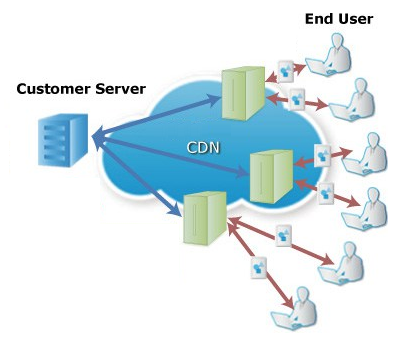
\includegraphics{pi2}
    \end{figure}
\newpage
\chapter {Introduction}
\section {DoS}
\hfill \break \gls{DoS} attacks are attempts to exhaust server-side assets and designed to prevent client-to-server communication (denial of service). Simply, we can say that stealth server sabotage wires or even the server is denial of service, but in the context of data security we discuss about remote attacks and not physical sabotaging.
\section {DDoS}
\hfill \break \gls{DDoS} attacks are very similar and sometimes even identical, and their intention is Distributed Denial of Service. In other words, the attack comes not from a single source, but from a large number of end stations – usually triggered by the attacker in the form of a king of virus located on these end stations. Most \gls{DDoS} attacks are much more powerful and significant. It is important to understand that even an attack by two or three end stations is usually considered as a \gls{DoS} attack, since there is really no significant flooding of the server.
\hfill \break Earlier this month Cisco released a white paper that \cite{corero} is part of the company’s larger report, “Visual Networking Index Complete Forecast Update, 2015-2020.” Here are some statistics from that white paper, relevant to distributed denial of service (\gls{DDoS}) attacks:
\begin{itemize}
\item Frequency of distributed denial-of-service (\gls{DDoS}) attacks has increased more than 2.5 times over the last 3 years.
\item	The average size of \gls{DDoS} attacks is increasing steadily and approaching 1 Gbps, enough to take most organizations completely off line.
\item	Peak \gls{DDoS} attack size (Gbps) is increasing in a linear trajectory, with peak attacks reaching 300, 400, and 500 Gbps respectively, in 2013, 2014, and 2015, at about 10 to 15 percent per year.
\item	In 2015 the top motivation behind \gls{DDoS} attacks was criminals demonstrating attack capabilities, with gaming and criminal extortion attempts in second and third place, respectively.
\item	\gls{DDoS} attacks account for more than 5 percent of all monthly gaming-related traffic and more than 30 percent of gaming traffic while they are occurring.
\item	Globally the number of \gls{DDoS} attacks grew 25 percent in 2015 and will increase 2.6-fold to 17 million by 2020.
\end{itemize}

\hfill \break The \gls{DoS} and \gls{DDoS} attacks can be divided into two types: 
\begin{itemize}
\item 	Attacks that flood and delay the service.
\item	Attacks that completely disrupt the service (and these we want to deal with in our project).

\end{itemize}
\begin{figure}
  \centering
        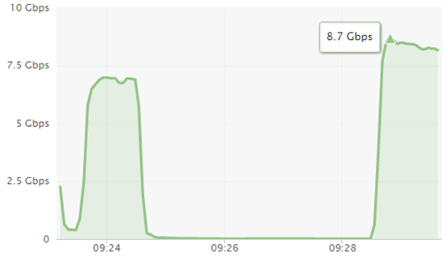
\includegraphics{ddos-attack-traffic-gbps}
	\caption{Sudden increase in server network traffic}
    \end{figure}

\section{DoS and DDoS attacks}
Our research is including both types of attacks for \gls{DoS} and \gls{DDoS} attacks in general, and we will divide the types into different main types, based on the seven-layer-model (\gls{OSI}) \cite{QuickGuide}.
\subsection {DoS and DDoS over Application layer} 
 \hfill \break Attacks in the application layer are often generated by POST requests. They are also divided to sub protocols in the application layer – http / https.
\begin{itemize}
\item\underline {HTTP POST Flood} 
- Creating and sending very large number of POST methods, to the extent that the server can't answer all requests, therefore service for real users of the server is compromised.

\item\underline{HTTPS POST Flood} - This is a flood of post methods that pass through \gls{SSL} Session. The purpose of \gls{SSL} is to take every message and decrypt it in order to inspect it. Flooding of these methods would harm the service.
\newpage
\item\underline{HTTP GET Flood} - The attacker creates and sends to the server a huge amount of GET requests. The server needs to analyze all of them and return some data. Some people regard this attack as a Transport-layer attack, since sometimes the server would have to send a lot of data to the user attacker. Therefore, traffic and network bandwidth are flooded. Denial and service prevention depends on the server’s capacity to getting and sending back packets. If it is able to handle a huge number of requests – the traffic will be damaged, and if it fails, the requests that it receives from real users will not be handled as the server falls.

\item\underline{HTTPS GET Flood} - Overflow of GET requests on HTTPS protocol requires a lot of work from \gls{SSL} Session – decryption every message and hence load and sabotage the service.
\end{itemize}
\hfill \break
\subsection {DoS and DDoS over Transport layer} 

 Flooding over Transport layer characterized mainly by packets that the server receives and is required to provide service – mostly by sending a requested data or any other response\cite{QuickGuide}.
\begin{itemize}
 \item\underline{Syn Flood} - In this attack, the attacker takes advantage of the \gls{TCP} principles that the server always wants to reach. When a server receives a Syn packet, it is a request from a client to open a connection, and it is obligated to respond to it and must return the client a Syn – Ack certificate. Each Syn message requires time from the server – analyzing the packet (understanding who created it, calculating ‘Check-sum’ etc.), and then be able to reply. Therefore, flooding these messages is slowing down and compromising the server’s serviceability.

\item\underline{Rst Flood} - Like Syn flood, the attacker takes advantage of \gls{TCP} principles, including reliable communication. In case that a socket is closed or when one of the sides disconnected (and in few other situations), \gls{TCP} has a solution. The connected side still wants to continue the communication (since there was no closing connection process), it sends a packet with a Rst flag and hence they have to re-open the connection. Like Syn packets overflowing, Rst packets overflowing also require a lot of work from the server and would sabotage the service.

\item\underline{\gls{UDP} Flood} - \gls{UDP} floods are used frequently for larger bandwidth \gls{DDoS} attacks because they are connectionless and it is easy to generate \gls{UDP} messages from many different scripting and compiled languages. The attack can be initiated by sending a large number of \gls{UDP} packets to random ports. As a result, the server would check for the application listening at that port, realize that no one is and reply with \gls{ICMP} packet saying ‘Destination Unreachable’. Thus, for a large number of \gls{UDP} packets, the server will be forced into sending many \gls{ICMP} packets and much performance.
\end{itemize}
\newpage
\subsection {DoS and DDoS over Network layer} 

 \hfill \break \gls{DoS} and \gls{DDoS} attacks over the Network layer are characterized with a large number of packets in order to overload the bandwidth and exhaust network resources. Network resources can be routers, firewalls and servers, and it is clear that their ability is final.
\begin{itemize}
\item\underline{\gls{ICMP} Flood} - \gls{ICMP} protocol is typically used for error messages rather than data exchange between systems. Flooding messages with \gls{ICMP} protocol – e.g. ping – is intended to overload the network.
\end{itemize}
 \hfill \break
\subsection {DoS and DDoS over Link layer}  

 \hfill \break \gls{DoS} and \gls{DDoS} attacks over the Network layer require access to the local network. Therefore, they are rare and more easy to detect.
\begin{itemize}
\item\underline{\gls{MAC} Flood} - A rare attack, in which the attacker has to be connected to the local switch. The attacker sends multiple dummy Ethernet frames, each with different invalid \gls{MAC} address. Network switches maintaining their \gls{MAC} table, and treating \gls{MAC} addresses separately, and hence reserve some resources for each request. When all the memory in the table is used up, it either shuts down or becomes unresponsive.
\end{itemize}


 \hfill \break
\subsection {Demonstrating APDoS Attack}

 \hfill \break  \gls{APDoS} is an attack that combines many \gls{DoS} and \gls{DDoS} attacks, and is carried out by a lot of hostile elements over time. \gls{APDoS} represents the worst Denial of Service attack that can occur. The idea behind it is a combination of many attacks from multiple endpoints, and over long period of time, hence its name Advances Persistent \gls{DoS}. In this attack, the attackers usually attack several stations in order to create a distraction from the \gls{DoS} defenses, but concentrate on one main victim in the organization.
\newpage
\section{DoS and DDoS defense solutions }

\subsection{DoS and DDoS solutions over Application layer}
 
\begin{itemize}
\item\underline {HTTP POST Flood} -  There is a difficulty in distinguishing between legal traffic and attack.
The most effective mechanism that exists today is by combining methods of characterizing the movement of requests and identifying the source user.
When a random url is used, an exception check is required to understand that this was an attack and not an innocent use of the server \cite{AppstSolution}. Part of the exception check is to try to identify the source user that triggers the attack, and you may notice that sometimes a large part of the package signature and content is the same.

\item\underline {HTTPS Request Flood} - Using the BIG-IP system \cite{HTTPSRequestSolution} and the F5 iRules scripting language.
Now available via the F5 DevCentral online community, this iRule states that if a device tries to renegotiate more than five times in any 60-second period, the connection is silently dropped.
The biggest benefit to this approach is that the attacker believes the attack is still working and in service, when in actuality, the server has ignored the request and moved on to processing valid user requests instead.


\item\underline {HTTP GET Flood} Today We know about two detection algorithms \cite{AppstSolution}, one is focusing on a browsing order of pages and the other is focusing on a correlation with browsing time to page information size. that implement detection techniques and evaluate attack detection rates, i.e., false positive and false negative. The results show that our techniques can detect the HTTP-GET flood attack effectively.
\end{itemize}

\subsection {DoS and DDoS solutions over Transport layer} 
\begin{itemize}
\item\underline{Syn Flood} - We have a lot of solution \cite{SynSolution} for this attack:
Filtering ,Increasing Backlog,Reducing SYN-RECEIVED Timer,Recycling the Oldest Half-Open \gls{TCP},SYN Cache,SYN cookies,Hybrid Approaches,Firewalls and Proxies
We will expand a bit on SYN cookie is a technique used to resist SYN flood attacks. The technique's primary inventor Daniel J. Bernstein defines SYN cookies as "particular choices of initial \gls{TCP} sequence numbers by \gls{TCP} servers." In particular, the use of SYN cookies allows a server to avoid dropping connections when the SYN queue fills up. Instead, the server behaves as if the SYN queue had been enlarged. The server sends back the appropriate SYN+ACK response to the client but discards the SYN queue entry. If the server then receives a subsequent ACK response from the client, the server is able to reconstruct the SYN queue entry using information encoded in the \gls{TCP} sequence number.

\item\underline {Rst Flood} - A RST packet is accepted if the sequence number is in the receiver's window, or when a connection is closed (closed socket). This is slightly different from a FIN, which just says that the other endpoint will no longer be transmitting any new data but can still receive some.

There are three types of event that cause a RST to be emitted. A) the connection is explicitly aborted by the endpoint, e.g. the process holding the socket being killed (just closing the socket normally is not grounds for RST, even if there is still unreceived data). B) the \gls{TCP} stack receiving certain kinds of invalid packets, e.g. a non-RST packet for a connection that doesn't exist or has already been closed. C) An unexpected amount of RST packets gained and there is no stopping point when sending back even a few responses.
Emmiting these senarios would mitigate the performance and engagement of the server with unwanted traffic. \cite{RstSolution}.
\end{itemize}

\subsection {DoS and DDoS solutions over Network layer} 
\begin{itemize}
\item\underline {\gls{ICMP} Flood} - Reconfiguring your perimeter firewall to disallow pings will block attacks originating from outside your network, albeit not internal attacks \cite{ICMPSolution}. Still, the blanket blocking of ping requests can have unintended consequences, including the inability to diagnose server issues.
The Incapsula \gls{DDoS} protection provide blanket protection against \gls{ICMP} floods by limiting the size of ping requests as well as the rate at which they can be accepted.
\end{itemize}
 \hfill \break

\subsection {APDoS solution}

 \hfill \break To combat \gls{APDoS}, organizations require a single vendor, hybrid cyber security solution that protects networks and applications from a wide range of attacks. Ideally, such a solution \cite{APDoSSolution} includes all the different technologies needed for effective detection and mitigation, including \gls{DoS}/\gls{DDoS} protection, behavioral analysis, \gls{IPS}, encrypted attack protection and web application firewall (WAF). Additionally, organizations also require new levels of partnership with their \gls{DDoS} mitigation service provider and any \gls{ISP} that provides managed \gls{DDoS} services to coordinate for the effective detection and mitigation of a multi-vector assault.

\newpage
\chapter {Related Work}
\section {Related Articles}
\subsection {Traffic flooding attack detection with SNMP MIB using SVM}
\gls{DoS} and \gls{DDoS} attacks have become more and more destructive, and are threatening to various network services. Hence, the various methods of protection and monitoring and control of network traffic have also begun.
However, most of the current modern detection systems are focusing on detail analysing for each packet’s data, which causes late detection and can’t handle high network traffic.
  \hfill \break
 \gls{SNMP}\cite{snmp}  provides a universal method of exchanging data for purposes of monitoring systems that reside on a network. The use of  \gls{SNMP} is most dominant in the modern industry. But, to utilize  \gls{SNMP} for traffic flooding attack detection, we need to consider the following three points in the use of the  \gls{SNMP} MIB variables which affects the performance and accuracy of the detection system:
\begin{itemize}
\item Proper selection of  \gls{SNMP} MIB variables for attack detection
\item Determination of the detection timing about when and how often
\item Algorithm for attack detection using the selected MIB (Management Information Base) variables.
\end{itemize}
  \hfill \break

\subsection {Change trend of averaged Hurst parameter of traffic under DDoS flood attacks}
\gls{DoS} and \gls{DDoS} flood attacks are great threats to the internet though various approaches and systems have been proposed. Hence, Intrusion Detecting System (IDS) and Intrusion Preventing System (\gls{IPS}) are desired. The \gls{DDoS} flood attack sends packets upon a server with a huge amount of traffic. It never tries to break into the server’s system, which makes the servers’s security defenses irrelevant.
\hfill \break
The solutions given by misuse detection are primarily based on a library of known signatures to match against network traffic . Hence, unknown signatures from new variants of an attack mean are hard to be recognized. Therefore, anomaly detectors (exceeded routine detectors) play a role in detection of \gls{DDoS} flood attacks.
\hfill \break
It is important considering the Hurst parameter - H in characterizing exceptions of traffic series in packet size under DDOS flood attacks. This paper specifically  \cite{Hurst} studies how H of traffic is changing under \gls{DDoS} flood attacks. It it important understanding the following:
\begin{enumerate}
\item Whether H of traffic when a server is under \gls{DDoS} flood attacks is much different from the regular one?
\item How is H changes when a server suffers from \gls{DDoS} flood attacks?
\end{enumerate}
Answering these questions might give us better understanding for detecting and protecting from \gls{DDoS} flood attacks.
\hfill \break

\subsection{Software-Defined Networking (SDN) and Distributed Denial of Service (DDoS) Attacks in Cloud Computing Environments }
Cloud computing develops rapidly due to its essential characteristics. Cloud computing would not be possible without the underneath support of networking. Recently, \gls{SDN}  \cite{SDN} has attracted great interests as a new paradigm in networking. In \gls{SDN} , network intelligence and state are logically centralized, and the underlying network infrastructure is abstracted from the applications. Denial of Service (\gls{DoS}) attacks and Distributed De-
nial of Service(\gls{DDoS}) flooding attacks are the main methods to destroy availability of cloud computing.
Although the capabilities of \gls{SDN}  make it easy to detect and to react\gls{DDoS} attacks in cloud environments, the separation of the control plane from the data plane in \gls{SDN}  introduces new attack planes. \gls{SDN}  itself may be a target of some attacks, and potential \gls{DDoS} vulnerabilities exist across \gls{SDN}  platforms. For example, an attacker can take advantages of the characteristics of \gls{SDN}  to launch \gls{DDoS} attacks against the control layer, infrastructure layer plane and application layer of \gls{SDN} .
 \hfill \break
\section {Related Productions}
\subsection {Cisco - 'DDoS Mitigation' } 
Cisco had developed a System which delivers a complete \gls{DDoS} protection solution based on the principles of detection, diversion, verification, and forwarding to help ensure total protection\cite{cisco}. The solution maintains the business continuity by: 
\begin{itemize}
\item Detecting the \gls{DDoS} attack.
\item Diverting  the data traffic destined for the target device to  a Cisco appliance for treatment.
\item Analyzing and filtering  the bad traffic flows from the good traffic flows packets, preventing malicious traffic from impacting performance while allowing legitimate transactions to complete.
\item Forwarding  the good traffic to maintain business continuity.
\end{itemize}
\newpage
\subsection {Check Point -  'DDoS Protector' }
Check Point had developed a System called '\gls{DDoS} Protector'\cite{checkpoint}, which keeps businesses running with multi-layered, customizable protections and up to 40Gbps performance that automatically defends against network flood and application layer attacks with fast response time against today’s sophisticated denial of service attacks.
\hfill \break
\gls{DDoS} Protector Appliances offer flexible deployment options to easily protect any size business, and integrated security management for real-time traffic analysis and threat management intelligence for advanced protection against\gls{DDoS} attacks.
The product provides multi-layer protections, handles network and traffic flood and has a management system.
  \hfill \break
\subsection {Our work }
In order to implement our system, we will must focus on preventing the  \gls{DoS} and \gls{DDoS} attacks from our side.\hfill \break
Similar to `doi` system (Traffic flooding attack detection with \gls{SNMP} MIB), we have to analyze the traffic coming from the network, \hfill \break
 and to determine which traffic and data are meant to harm our system. Just like they did, we must realize which second third and more identical packets are caused due to timeouts or part of some \gls{DoS} or \gls{DoS} attacks.\hfill \break
In contrast, determining which `H` traffic is under \gls{DDoS} flood attack, in our opinion won't help us developing a system which would prevent our server to handle requests.\hfill \break
In addition we note that no other related workers implemented their system upon a \gls{CDN} server which is separated from the server. \hfill \break
This is a very important point because our whole goal is to assist our server in cases of \gls{DDoS} attacks.\hfill \break
 If the server would analyze the requests arriving and running our algorithm, he will not be able to handle the requests themselves. \hfill \break
 Remember, the server might deal with its databases, algorithms and even complex calculations. The server hypothesis should be that most of the requests are legal and not meant to harm it. \hfill \break
Thats where our system's importance.
In order to manage building a proper solution for \gls{DoS} and \gls{DDoS} traffic flood attacks, the system must contain the following:
\begin{itemize}
\item A durable \gls{CDN} server which could communicate both with the server and the clients.
\item Proper algorithm which can identify traffic status and mark and block specific ips and subnets.
\item Experiment \gls{DoS} and \gls{DDoS} attacks with and without our algorithm in order to determine that our algorithm is properly working and mitigation any attack.
\end{itemize}
\newpage
\chapter {Difficulties}
When we developed and even planned our system, we had a few technical and theoretical issues. 
\section {Building our own system}
In order to determine the specific behavior and requests handling of the server, we must develop our server:
\begin{itemize}
\item Coding a server which listens and handles every request properly.
\item Developing a \gls{CDN} server, which accepts requests from clients, following them to the server, and when answer from the server arriving, return it to the right client from many clients.
\item Coding a client end-point which could send regular request or multiple flooding requests over the server.
\item Developing an algorithm which can identify and analyze the requests and deciding either to handle the request, mark the specific client, or block it.
\end{itemize}
\section {Creating a proper network environment}
In addition, to determine that our system really providing a proper solution for \gls{DoS} and \gls{DDoS} attacks, we had to implement such attacks:
\begin{itemize}
\item Creating a network simulation of our network architecture.
\item Use it in a third-party application which could demonstrate a real \gls{DoS} and \gls{DDoS} attacks.
\end{itemize}
\section {Experimenting the system}
After planning, developing and using our system, we should decide if it is good enough for a proper solution for web servers. Our goal is to provide continuous activity of the server even when it is under \gls{DoS} or \gls{DDoS} attack.
\begin{itemize}
\item Experimenting our system, and analyzing it against other existing solutions.
\item Integrating our system with existing web servers.
\end{itemize}
\section {Future difficulties}
Beyond our project, there is a whole world of \gls{DoS} and \gls{DDoS} attacks. In our future progressive work, we need to give other solutions to a variety of \gls{DoS} and \gls{DDoS} attacks:
\begin{itemize}
\item Building a mitigation for other layers except Application-Layer (e.g. Transport-Layer).
\item Making our system available even for apache servers and not only web or desktop servers.
\item Determining which is the best platform for mitigating \gls{DoS} and \gls{DDoS} attacks - \hfill \break Asynchronous single-threaded or Synchronous multi-threaded. There are many difference opinions in this case.
\end{itemize}
\newpage
\chapter {Our algorithm}
\section {Calculating approved count of times for each file}
\label{sec:algo1}
  \begin{algorithm}
   \caption{}
    \begin{algorithmic}[1]
      \Function{Max-file-requests}{$file$}
        	\State Let smallestFile be the smallest file in the server
	\State Let smallestCount be his number of approved requests for it.
	\State Let biggestFile be the smallest file in the serverr
	\State Let biggestCount be his number of approved requests for it.
            \If {$ file == biggestFile$}
                 \State \Return return biggestFile
            \ElsIf {$ file == smallestFile$}
                \State \Return return smallestFile
            \Else
              	\State Let y be the ratio between the files: $y=\dfrac{file-small}{big - small} $
	 	\State Let expectedCount be number of ratio between them:
  		\State $ansRequest=smallRequest-  \dfrac{(smallRequest-bigRequest)*Y}{100}$
		\State $expectedCount = round( expectedCount )$
	  	\State \Return expectedCount
            \EndIf
       \EndFunction
\end{algorithmic}
\end{algorithm}
\newpage
\section {Handle request for tracking table}
Define tracking-table (ip, file, time, count)
Define max-time – maximum time between several requests
  \begin{algorithm}
   \caption{}
    \begin{algorithmic}[1]
      \Function{Handle-track-table}{$ip, file, time$}
        	\State Let ip be the requested ipr
	\State Let file be the requested file
	\State Let time be the current time
            \If {$ tracking-table [ ip ] !=   null$}
                 	\State $count \leftarrow 1$
 		\State  Insert to the table: ip, file, time, count	
            \ElsIf {tracking-table [ ip ] not contains file}
                     \State $count \leftarrow 1$
 		\State  Insert to the table: file, time, count	    
            \Else
              	\State Let firstTime be the first time the ip requested this file.
		 \If {$ | firstTime – time | $ $>$  $max-time $}
                 		\State $tracking-table [ ip ] [ time ]  \leftarrow time$
                 		\State $tracking-table [ ip ] [ count  ]  \leftarrow 1$
            	\Else
                     		\State $count++$
 			\If {$count$ $>$ $max-file-requests ( file )$}
		 	\State \Return false
			\EndIf
		\EndIf
	\EndIf
  	\State \Return true
       \EndFunction
\end{algorithmic}
\end{algorithm}
\newpage
\section {Handle request}
Define blocking-table: ( ip, ExpIncreament, degree )
  \begin{algorithm}
   \caption{}
    \begin{algorithmic}[1]
      \Function{Blocking-IP}{$ip, file, time$}
            \If {$ blocking-table [ ip ] != null$}
                 	\State Close the socket
            \ElsIf {$Handle-track-table( ip, file, time ) == false$ }
                     \State blocking-table [ ip ] [ ExpIncreament ] ++

            \If {$ExpIncreament >= 3 $}
                 	\State Block user
	\Else
 		\State  blocking-table [ ip ] [ degree ] $\leftarrow 2^ {ExpIncreament}$
	\EndIf	    
            \Else
              	\State Handle the request
	\EndIf
       \EndFunction
\end{algorithmic}
\end{algorithm}

\section {Intervals}
  \begin{algorithm}
   \caption{Intervals}
    \begin{algorithmic}[1]
           \State Every 15 seconds downgrade every degree.
	\State Every 3 minutes reset all tables.       
\end{algorithmic}
\end{algorithm}


\section {Advantages and disadvantages }
\subsection{Advantages}

\begin{itemize}
\item Working on every server platform (web servers, desktop server or cloud servers).
\item Does not require a specific operating system.
\item Does not requires any external packages.
\item Calculating blocking users together with requested file sizes.
\end{itemize}
\subsection{Disadvantages}

\begin{itemize}
\item Taking time to implement.
\item Protective only for Application-layer (\gls{OSI}).
\end{itemize}

\chapter {Related mitigations}
\section {Mod evasive}

\subsection {Explanation}
mod evasive is a module for Apache that provides evasive action in the event of an \gls{HTTP} \gls{DoS}  or \gls{DDoS}  attack or brute-force attack. \hfill \break
The module tracks  \gls{HTTP} connections and verifies how many requests for a page are done within a given time frame. If the number of concurrent requests exceeds a specified threshold, then the request is blocked. This blocking is done on an application level. The requester gets a forbidden answer to the request. \hfill \break
It allows you to add your management and proxy networks to the DOSWhitelist setting so that you do not block your own network.
\subsection {How to use}
On Ubuntu, run:
\begin{lstlisting}[frame=single]
$ sudo apt-get install libapache2-mod-evasive
$ sudo mkdir /var/log/mod_evasive       // creating log folder
$ sudo a2enmod evasive                  //enabling mod_evasive
\end{lstlisting}

\subsection {Advantages and disadvantages }
\subsubsection{Advantages} 
\begin{itemize}
\item Very easy to use.
\item Very effective.
\end{itemize}
\subsubsection{Disadvantages}
\begin{itemize}
\item Working only on Apache servers.
\item External package use.
\item Requires Ubuntu operating system only.
\item Protective only for Application-layer (OSI).
\end{itemize}
\newpage
\section {Information security / network-layer approach}

\subsection {Explanation}
A far more practical way, considering we are deciding for the fate of the packet right before it reaches the other end or even if it had already completed the 3-way handshake. consider these examples:\hfill \break
a. restrict the number of concurrent connections per IP on your firewall. this will give you the ability to define how many connections can a client requests simultaneously.
in iptables, you can do this by:
\hfill \break

\begin{lstlisting}[frame=single]
$  iptables -p tcp --syn --dport 80
   -m connlimit --connlimit-above 20
   --connlimit-mask 24 -j DROP
\end{lstlisting}

in openbsd, you can do this in pf.conf:

\begin{itemize}
\item Limit the absolute maximum number of states that this rule can create to some number (e.g. 200)
\item Enable source tracking; limit state creation based on states created by this rule only
\item Limit the maximum number of nodes that can simultaneously create state to some number (e.g. 100)
\item Limit the maximum number of simultaneous states per source IP to 3
\end{itemize}
\hfill \break
Example in bash (OpenBSD operating system):

\begin{lstlisting}[frame=single]
pass in on $ext_if proto tcp to $web_server \
     port www keep state \
     (max 200, source-track rule, max-src-nodes 100, max-src-states 3

\end{lstlisting}


\subsection {Advantages and disadvantages }
\subsubsection{Advantages} 
\begin{itemize}
\item You’re preventing the attack even before it arrived to the 3-way-handshake.
\item Quite easy to implement.
\end{itemize}
\subsubsection{Disadvantages}
\begin{itemize}
\item You need to know the average amount of users per hour.
\item You might limit some users when not needed.
\item Access to the ip-tables required.
\end{itemize}

\chapter {Technical work}
\section {Our systems}
\subsection {Building our own server and CDN server}
In order to determine the specific behavior for the \gls{CDN} server and original server when packets are arriving, we had to code our own servers. This was expressed in the following cases:
\begin{itemize}
\item Paying attention in every type of http request, (text/plain , text/html , application/javascript etc.).
\item The server had to calculate the file sizes and give priority for each one of them.
\item The \gls{CDN} server should gain the priority table, and to mark significant users from flooding the server. In addition it should close the socket for every flooding user, and to count it.
\item Determining which end-point is a non-regular user, and be able to block it if needed.
\item Creating registration for gained requests, and thus we were able to experiment our system.

\end{itemize}
For that, we used NodeJS platform for building the servers. Asynchronous single threaded servers are usually very fast than regular servers, and that helped us to handle huge amount of request per second.

Usage: node Client [options]

\begin{lstlisting}[frame=single]
$ node server --port <port>

   Flags:
  --port             define argument of PORT listener.

   Args:
  <port>             Port value for server's listener.
\end{lstlisting}

Usage: node Server [options]

\begin{lstlisting}[frame=single]
$ node request -t <ip> -p <port> -f <path> -ht <requested file>

  Flags:
  -t                  define argument of IP destination.
  -p                  define argument of Port destination.
  -f                  define argument of path folder.
  -ht                 define argument of requested file

  Args:
  <ip>                IP address for attack.
  <port>              Port destination for attack.
  <path>              path of folder to download files
		      (default /dev/null/)
  <requested file>    path to requested file on the server.
\end{lstlisting}

\newpage

Usage: node CDN [options]

\begin{lstlisting}[frame=single]
$ node CDN --server <server_ip> --serverPort <server_port> 
  --port <port> --no-protect 
  Flags:
  M  - Mandatory
  --port              define CDN server's port argument 
		      (4400 by default)
  --server       M    define original server's IP argument
  --serverPort   M    define original server's Port argument
  --no-protect   M    define CDN mitigation

 Args:
  <server_ip>          IP address of Server.
  <server_port>        Port destination for server
  <port>               Port destination for CDN.
\end{lstlisting}

\subsection{Create System}
We are discussing and investigating all about \gls{DoS} and \gls{DDoS} attacks. In order to really simulate a \gls{DDoS} attacks, we need several different end-points to flood our servers. Create system do just that.\hfill \break
With NS file system (Network simulator), we’re creating virtual nodes representing our server, \gls{CDN} sever, and clients. This language was built in order to simulate virtual nodes and be able to link between them – creating virtualized vetwork.\hfill \break
On each end-point we installed Ubuntu (Linux Distribution), and on each one of them installed NodeJS. The nodes on Create system are not connected to any external network, thus the have no internet connection. In order to install it we had to define Create’s proxy connection and then we were able to get the external files.\hfill \break
Because these nodes are virtual, there is no real built-in gateway on the router, and for each end-point we need to simulate a router and a gateway in order to route packets to the right direction.\hfill \break
\hfill \break
\noindent  
Example for node set up:
\hfill \break
\begin{lstlisting}[frame=single]
$ tb-set-node-os $server Ubuntu1404-32-STD
$ set routerServer [$ns node]
$ tb-set-node-os $routerServer Ubuntu1404-32-STD
$ set link55 [$ns duplex-link $routerServer $gatewayServer 
  1000Mb 0ms DropTail]
$ set MainLink [$ns make-lan "$gatewayCDN $gateway1 $gateway3
  $gateway2 $gatewayServer " 100Mb 0ms ]
\end{lstlisting}


In addition, we simulated one link, which will represent a huge connected system between several end-points.

 \par
        \begin{minipage}{\linewidth}
            \centering
            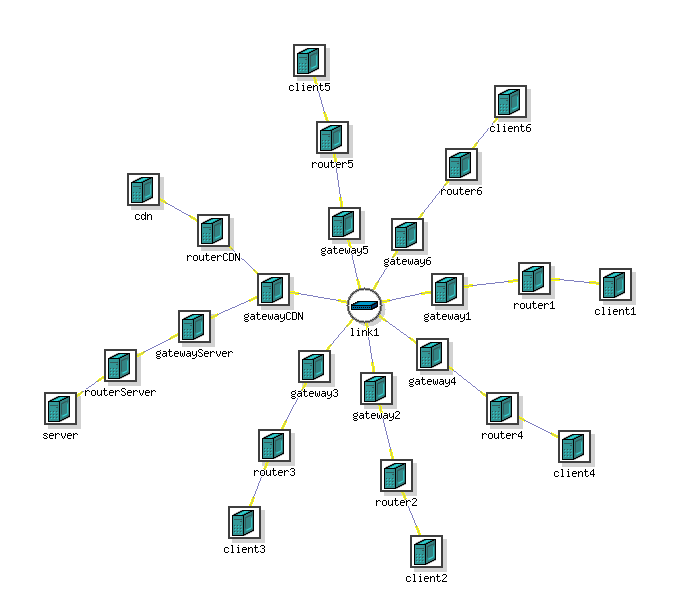
\includegraphics[scale=0.5]{ns}
            \captionof{figure}{Gateways in general are being provided for each router, but when defining virtual routers, they are our way to route packets to the right end-point.}
        \end{minipage}


\section {Experiments} 
After implementing our system, we’ve made many experiments in order to test and prove our system’s success with mitigating \gls{DDoS} attacks. For each experiment, we first turned on the servers, and then started to run the client sides.
\begin{enumerate}
\item\underline {Multiple end-points without any mitigation}:
The server gained in average ~3600 requests in 3 seconds (~1200 per second). After 12 seconds of flooding, the server was shut down.  \hfill \break  \hfill \break
        \begin{minipage}{\linewidth}
            \centering
            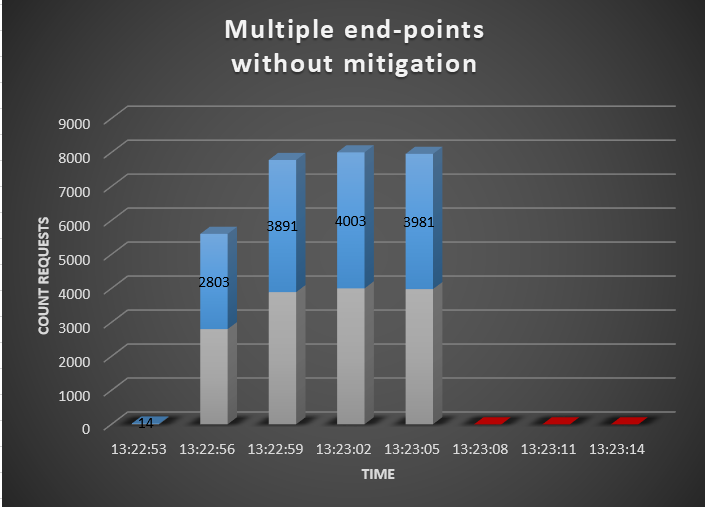
\includegraphics[width=10cm,height=7cm,keepaspectratio]{multi_without}
            \captionof{figure}{\gls{DDoS} traffic flood attacks without our mitigation.}
        \end{minipage}
 \hfill \break
\item\underline {Single end-point without mitigation}:
The server gained in average ~2000 requests in 3 seconds (~670 per second). The server could handle all of the request although the huge amount.  \hfill \break  \hfill \break
        \begin{minipage}{\linewidth}
            \centering
            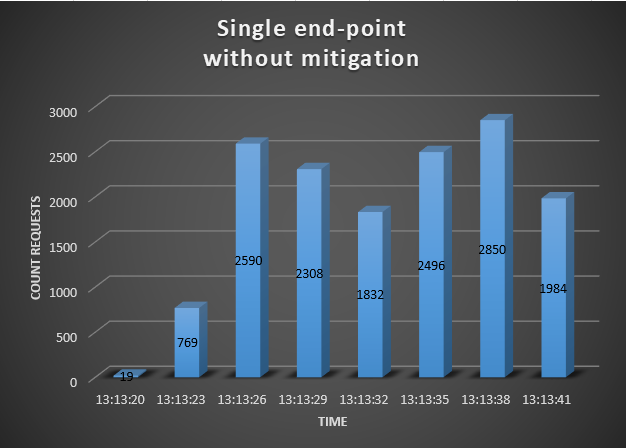
\includegraphics[width=10cm,height=8cm,keepaspectratio]{single}
            \captionof{figure}{\gls{DoS} traffic flood attacks without our mitigation}
        \end{minipage}
\item\underline {Multiple end-points with our mitigation}:
he server gained in average ~55 requests in 3 seconds (~18 per second). No significant flood on the server.  \hfill \break  \hfill \break
     \begin{minipage}{\linewidth}
            \centering
            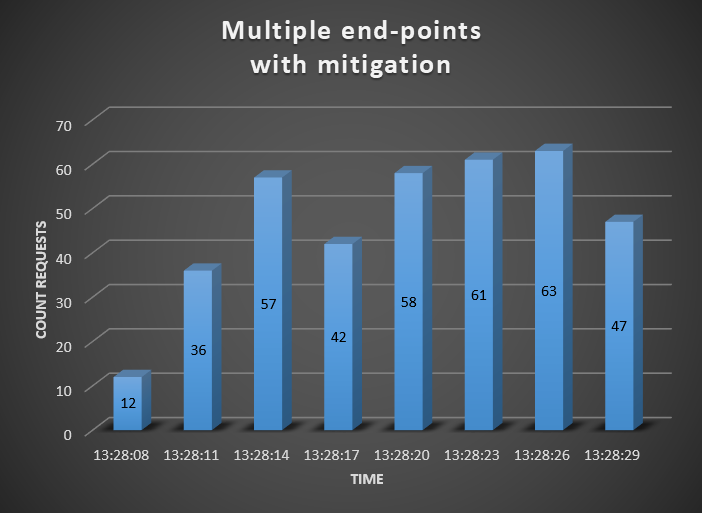
\includegraphics[width=10cm,height=8cm,keepaspectratio]{multi_with}
            \captionof{figure}{\gls{DDoS} traffic flood attacks with our mitigationn}
        \end{minipage}
 \hfill \break
\end{enumerate}
\newpage
\section {Our Innovation - Conclusion} 
\gls{DoS} and \gls{DDoS} protections have existed for many years, and many companies know how to respond to a variety of attacks. Also for Application-Layer (\gls{OSI}) flood attacks, many mechanisms of companies that specialize in protections for web servers, contains also a protection for these attacks.\hfill \break
However, there is no protection intended only for Application-Layer (\gls{OSI}) flood attacks, and an attack that can be so simply done (a few lines of code), requires a specific protection without any enveloping system.\hfill \break
Our only preoccupation with Application-Layer (\gls{OSI}) flood attacks is unparalleled on the net, and no company is dealing only with Application-Layer (\gls{OSI}) flood problem. In this situation, many web servers may lose the ability to serve customers easily, and only answer thousands of dollars of a large system that will protect the site from attacks that would probably never arrive.\hfill \break \hfill \break
In order to build our system, we successfully meet the following requirements:\hfill \break

\begin{itemize}

\item Investigating what is \gls{DoS} and \gls{DDoS} attacks, and focusing on Application-Layer - http flood attacks.
\item Researching about other existing solutions, learning from other companies which already invented such defenses / algorithms.
\item Developing our own servers (regular and \gls{CDN}), and end-points representing clients or attackers.
\item Testing and experimenting our system with several tools - Integration tools and multi - end points servers to demonstrate a real \gls{DoS} or \gls{DDoS} attack.
\item `Post Mortem` - Analyzing the results - does our system give a proper solution for web servers?

\end{itemize}

We note that our system has a few innovations that no other company implemented. It starts with the \gls{CDN} implementation. Each one of them used their system within the original server. It means that their server should focus both on mitigating any \gls{DoS} or \gls{DDoS} attack, and also continue serving its clients properly and all that implies (interpret each request, deal with the databases and to perform complex calculations).\hfill \break
In addition, each one of our related workers considered the amount requests coming from an end-point. Our mitigating algorithm considers both the amount of requests and the specific request. This means that when the request has a minor significance in meaning of server calculations and network traffic, it will get the same treatment in our mitigating algorithm.\hfill \break (see our \hyperref[sec:algo1]{calculation file algorithm})



\newpage
\section {Developing environment }

\subsection {Git}
     \begin{minipage}{\linewidth}
            
\includegraphics[width=1cm,height=1cm,keepaspectratio]{github}
        \end{minipage}
\hfill \break
In order to work in parallel and to maintain all the work we’ve done, we used git as our version control manager for the project, and GitHub as our git server containing our repository. It helped us to keep well organized work, reverting changes when mistaken and track each other work. \href{https://github.com/}{(link)} 

\subsection {Tests}
     \begin{minipage}{\linewidth}
            
\includegraphics[width=2cm,height=2cm,keepaspectratio]{jasmine}
        \end{minipage}
\hfill \break
In order to know that the project is working as expected, we wrote tests for each module, and each functionality of the project.\hfill \break
We used Jasmine as our test runner, a very conventional test runner.\hfill \break
Our project contains 57 tests – 52 unit tests and 5 integration tests.
\begin{itemize}
\item Unit tests are covering our utility functions – validators, filesystem requests and programming stuff.
\item Integration tests are covering our end-to-end tests: The whole steps since the server is on, \gls{CDN} server connects to the server, and the client sending requests for them.
\end{itemize}
The tests are helping us to determine that every time we’re pushing new code, the base code is still working as expected. \href{https://jasmine.github.io/}{(link)} 
\subsection {Lint}
     \begin{minipage}{\linewidth}
            
\includegraphics[width=2cm,height=2cm,keepaspectratio]{eslint}
        \end{minipage} \hfill \break 
Lint is a tool which helps us to manage our code validity, style and efficiency. As most of our project was built by NodeJS, we used ESLint as our Lint rule. Around ~30 rules are on for errors or warnings. \href{https://eslint.org/}{(link)} 
\subsection {CI}
     \begin{minipage}{\linewidth}
            
\includegraphics[width=1.5cm,height=1.5cm,keepaspectratio]{circleci}
        \end{minipage}
\hfill \break
Lint and tests are very good, but useless when a developer doesn’t run them every time he is writing new code. Continues Integration is obliging us to run our tests and lint rules before any merging our code into master branch. We used CircleCI tool in order to connect our GitHub repository and to run our Jasmine tests and ESLint rules for any new code.
\href{https://circleci.com/}{(link)} 


\newpage

\subsection {CREATE}
     \begin{minipage}{\linewidth}
            
\includegraphics[width=2cm,height=2cm,keepaspectratio]{create}
        \end{minipage}
\hfill \break
CREATE is a state-of-the-art scientific computing facility for cyber-security researchers engaged in research, development, and testing of innovative cyber-security technology. It helped us to simulate the \gls{DDoS} attacks over multiple end-points.
\href{https://https://create.iucc.ac.il/}{(link)} 

\subsection {NodeJS}
     \begin{minipage}{\linewidth}
            
\includegraphics[width=2cm,height=2cm,keepaspectratio]{js}
        \end{minipage}
\hfill \break
Node.js is an open-source, cross-platform JavaScript run-time environment that executes JavaScript code for servers and operation systems. With Node.js we’ve built our own server and \gls{CDN} server, and thus managed to determine our desirable behavior for handling packets.
\href{https://nodejs.org/}{(link)} 

\subsection {NS}
A network simulator is software that predicts the behavior of a computer network. With it we managed to simulate our large network and to make a real \gls{DDoS} attacks, from several end-points.
\href{https://www.isi.edu/nsnam/ns/}{(link)} 

\subsection {Tkinter}
     \begin{minipage}{\linewidth}
            
\includegraphics[width=1.5cm,height=1.5cm,keepaspectratio]{tkinter}
        \end{minipage}
\hfill \break
Tkinter is a Python open-source library for \gls{GUI} software. With it we’ve built a simple use for our attacks.
\href{https://docs.python.org/3/library/tkinter.html}{(link)} 

\newpage
\chapter {Future work}
We’ve done a huge research work, and built multiple modules that could handle \gls{DoS} and \gls{DDoS} attacks when needed.
However, we would like to suggest a few improvements for our system:
\begin{enumerate}
\item We would like to handle not only Application-layer \gls{DoS} and \gls{DDoS} attacks, but also attacks in transport-layer (Syn / Rst floods), and even on link-layer, dealing with routing tables, as some of our related workers did.
\item Within our algorithm, we would like to add “White List” – which would gain several ips or a whole subnet to ignore from mitigation. Might be effective for companies which would like to give access for internal employees. In addition, “Black List” could be effective too, or to prepare such mechanism if some client would request it.
\item To divide some implementations for web server, desktop servers and cloud servers. It might be effective when some special requests needed in each one of them.
\item To test implementations between node servers (Asynchronous Single Threaded), and other servers (Synchronous Multi-Threaded). What would give the best solution?
\item Future DoS and DDoS attacks – hackers are developing every day, and we need to be ready (and even predict) for future attacks.
\end{enumerate}


%Print the glossary
\newpage
\addcontentsline{toc}{chapter}{Acronyms}
\printglossary[type=\acronymtype,title=Acronyms]
\newpage
\bgroup
\hypersetup{linkcolor = black}
\addcontentsline{toc}{chapter}{Figures}
\listoffigures
\egroup
\newpage
\addcontentsline{toc}{chapter}{References}
\printbibliography[title=References]
\end{document}


